\newpage
\section{Suggested solutions: Frequency Response}

\begin{enumerate}
\item The impulse response for an LTI system is:
$$h(t)=\frac{42\sin(\omega_{c}t)}{\pi t}.$$
Let the input to the LTI system be a periodic signal with period $T=1$ of the form:
$$x(t)=\sum_{n=-\infty}^{\infty}\delta(t-n).$$

\begin{enumerate}[a)]
\item Given $x(t)$ we find the Fourier transform as follows, firstly, we know that the Dirac comb can be expressed as a Fourier series of:
$$x(t)=\frac{1}{T}\sum_{n=-\infty}^{\infty}e^{i\frac{2\pi nt}{T}}.$$
In this case, we have $T=1$, hence:
$$x(t)=\sum_{n=-\infty}^{\infty}e^{i2\pi nt}.$$
Thus, the Fourier series coefficients are $c_{k}=1$ for all $k\in\mathbb{Z}$. Then the Fourier transform is:
$$\hat{x}(\omega)=2\pi\sum_{n=-\infty}^{\infty}\delta(\omega-2\pi n).$$
A plot of the spectrum for $\hat{x}(\omega)$ is shown in Figure \ref{diractrain} in red.

\begin{marginfigure}[1cm]
    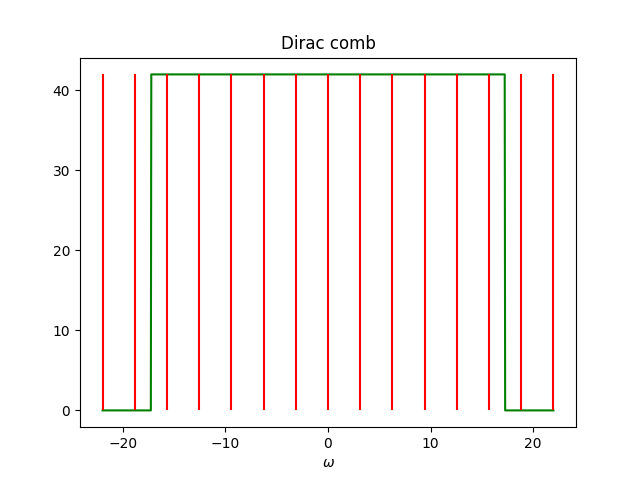
\includegraphics[height=7.5cm,width=7.0cm]{ch11/figures/diractrain.png}
    \caption{Spectrum for the Dirac comb between $-7\pi<\omega<7\pi$.}
    \label{diractrain}
\end{marginfigure}

\item The frequency response function is defined by:
$$\mathcal{H}(\omega)=\mathcal{F}\{h(t)\}=\int_{-\infty}^{\infty}\frac{42\sin(\omega_{c}t)}{\pi t}e^{-i\omega t}dt=42[u(\omega+\omega_{c})-u(\omega-\omega_{c})].$$
Figure \ref{diractrain} shows the frequency response in green.


\item The output of the LTI system can be found by convolution in time domain, that is $y(t)=h(t)*x(t)$, thus, 
in frequency domain we have multiplication by the convolution theorem. By Figure \ref{diractrain} the frequencies 
inside $(-5.5\pi,5.5\pi)$ remain after multiplication, but the frequencies outside $(-5.5\pi,5.5\pi)$ gets mapped to $0$. 

\item If $y(t)=c$ then $\hat{y}(\omega)=2\pi c\delta(\omega)$ so the frequency response must be such that:
$$2\pi c\delta(\omega)=\hat{x}(\omega)\mathcal{H}(\omega)=2\pi\sum_{n=-\infty}^{\infty}\delta(\omega-2\pi n)42[u(\omega+\omega_{c})-u(\omega-\omega_{c})]=2\pi42\delta(\omega),$$
the only way for this to work is that $|\omega_{c}|\le\pi$ giving $c=42$. 
\end{enumerate}

\item A running average filter is defined as:
$$y[n]=\frac{1}{M}\sum_{k=0}^{M-1}x[n-k].$$
We'll assume that $M$ is an odd number. 

\begin{enumerate}[a)]
\item The impulse response function is obtained by feeding a Dirac delta function into the LTI system, so if $y[n]=\mathcal{T}\{x[n]\}$, 
then $h[n]=\mathcal{T}\{\delta[n]\}$. Doing this, we find that:
$$h[n]=\frac{1}{M}\sum_{k=0}^{M-1}\delta[n-k].$$

\item The frequency response is the DTFT of $h[n]$, which gives:
\begin{align*}
    \mathcal{H}(\hat{\omega})&=\sum_{k=0}^{M-1}\frac{1}{M}e^{-i\hat{\omega}k}=\frac{1}{M}\frac{1-e^{-i\hat{\omega}M}}{(1-e^{-i\hat{\omega}})}
    =\frac{1}{M}\left(\frac{e^{-i\hat{\omega}M/2}(e^{i\hat{\omega}M/2}-e^{-i\hat{\omega}M/2})}{e^{-i\hat{\omega}/2}(e^{i\hat{\omega}/2}-e^{-i\hat{\omega}/2})}\right), \\
    &=\underbrace{\frac{1}{M}\frac{\sin(\hat{\omega}M/2)}{\sin(\hat{\omega}/2)}}_{D_{M}(\hat{\omega})}e^{-i\hat{\omega}(M-1)/2}.
\end{align*}
The sum, is evaluated using known formulas for geometric sums. 

\item If we have a system with impulse response $h_{\tau}[n]=\delta[n-\tau]$, then the frequency response is:
$$\mathcal{H}_{\tau}(\hat{\omega})=\sum_{k=-\infty}^{\infty}h[k]e^{-i\hat{\omega}k}=\sum_{k=-\infty}^{\infty}\delta[k-\tau]e^{-i\hat{\omega}k}=e^{-i\hat{\omega}\tau}.$$

\item The following code can be used to make the plot shown in Figure \ref{freq_responses}:
\lstinputlisting[language=Python, caption=Plotting the frequency response code,label=code14_2]{ch11/code/ex11_2.py}

As expected, the functions are identical. 
\begin{marginfigure}
    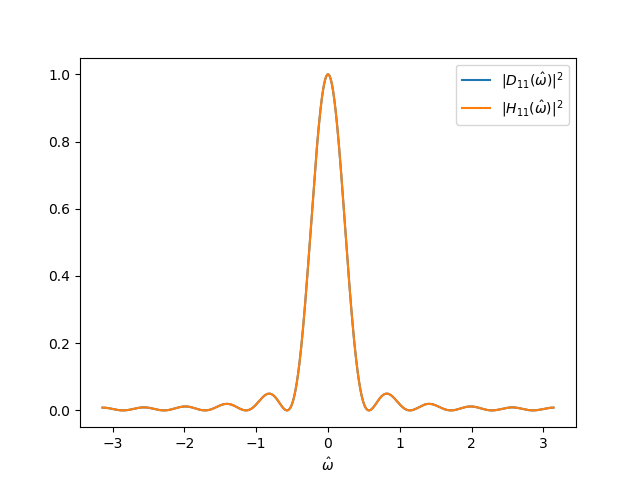
\includegraphics[height=7.0cm,width=7.5cm]{ch11/figures/frequency_responses.png}
    \caption{Comparison of frequency responses}
    \label{freq_responses}
\end{marginfigure}

\item The frequency response function was derived in b), and it has the form:
$$\mathcal{H}(\hat{\omega})=D_{M}(\hat{\omega})\mathcal{H}_{\tau}(\hat{\omega}),$$
where $\mathcal{H}_{\tau}(\hat{\omega})$ is a time-shift system with $\tau=(M-1)/2$. 

\item Claim: $|\mathcal{H}(\hat{\omega})|^{2}=|D_{M}(\hat{\omega})|^{2}$.
\begin{proof}
A simple computation gives:
\begin{align*}
    |\mathcal{H}(\hat{\omega})|^{2}&=\mathcal{H}(\hat{\omega})\mathcal{H}^{*}(\hat{\omega})=(D_{M}(\hat{\omega})\mathcal{H}_{\tau}(\hat{\omega}))(D_{M}(\hat{\omega})\mathcal{H}_{\tau}(\hat{\omega}))^{*},\\
    &=|D_{M}(\hat{\omega})|^{2}\underbrace{e^{-i\hat{\omega}\tau}e^{i\hat{\omega}\tau}}_{1}=|D_{M}(\hat{\omega})|^{2},
\end{align*}
as claimed. 
\end{proof}
In conclusion, both running average filters produce the same magnitude response, but one of them induces a time-shift while the other doesn't. 
\end{enumerate}

\item Consider an FIR filter approximation to the second derivative of the form:
$$h[n]=T_{s}^{-2}\delta[n+1]-2T_{s}^{-2}\delta[n]+T_{s}^{-2}\delta[n-1].$$

\begin{enumerate}[a)]
\item The frequency response can be found by the DTFT (Equation \ref{eq:fresp_ct}) as:
$$\mathcal{H}(\hat{\omega})=\sum_{k=-\infty}^{\infty}h[k]e^{-i\hat{\omega}k},$$
for this LTI system, we get:
$$\mathcal{H}(\hat{\omega})=T_{s}^{-2}e^{i\hat{\omega}}-2T_{s}^{-2}+T_{s}^{-2}e^{-i\hat{\omega}}=-2T_{s}^{-2}+T_{s}^{-2}2\cos(\hat{\omega})=\frac{2}{T_{s}^{2}}(\cos(\hat{\omega})-1).$$

\item The code shown in Listing \ref{code13_1} can be used to plot the spectral response. 
\lstinputlisting[language=Python, caption=Frequency response for finite difference,label=code13_1]{ex11_3.py}

Output of the code is shown in Figure \ref{spec_rep}.
\begin{marginfigure}
    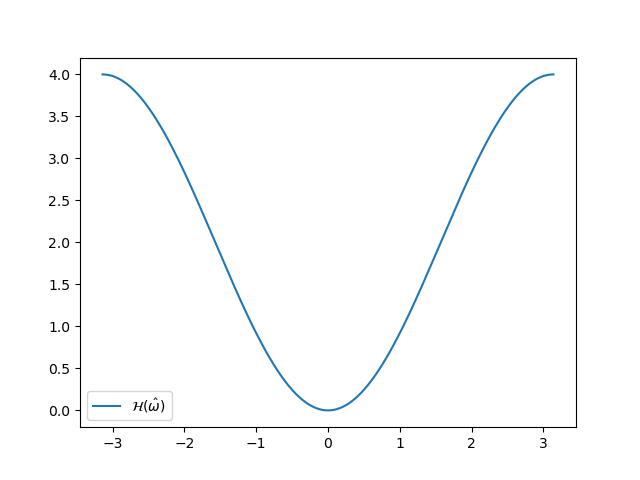
\includegraphics[width=7.0cm,height=6.5cm]{ch11/figures/freq13.png}
    \caption{Output of Listing \ref{code13_1}}
    \label{spec_rep}
\end{marginfigure}

\item In this case, the frequency response function is real, so the phase response is $0$. Meaning, there is no delay applied to the signal by this filter.

\item By looking at the plot of $|H(\hat{\omega})|$, we see that the filter is a high-pass filter, as the frequencies around $0$ are greatly reduced. 

\item Inspecting the plot, we see that for $\hat{\omega}=0$, the amplitude of the output signal will be $A'=0$. The reason is that in frequency domain we have:
$$\hat{y}(\hat{\omega})=\mathcal{H}(\hat{\omega})\hat{x}(\hat{\omega}).$$

\item The phase is not changed by the filter, so $\phi'=\phi$. For $\hat{\omega}=\pi/2$ the amplitude is doubled, so $A'=2A$, while for $\hat{\omega}=\pi$ the amplitude is scaled by $4$, giving $A'=4A$. 
This can be seen from the plot in Figure \ref{spec_rep} or by inserting the values into the frequency response function. 

\item The system $y(t)=\mathcal{T}\{x(t)\}=\frac{d^{2}}{dt^{2}}x(t)$ is a continuous-time LTI system, so:
$$y(t)=\mathcal{H}(\omega)x(t).$$
In particular, if we take $x(t)=Ae^{i\phi}e^{i\omega t}$, then:
$$y(t)=\frac{d^{2}}{dt^{2}}(Ae^{i\phi}e^{i\omega t})=Ae^{i\phi}(i\omega)^{2}e^{i\omega t}=-Ae^{i\phi}\omega^{2}e^{i\omega t}=-\omega^{2}(Ae^{i\phi}e^{i\omega t})=\mathcal{H}(\omega)x(t),$$
thus $\mathcal{H}(\omega)=-\omega^{2}$. 

\item Comparing the plots, we conclude that the approximation is only good for small angular frequencies in the range $0<\omega<\pi/2$. 
\end{enumerate}

\end{enumerate}


